\documentclass[letter]{bioinfo}

\copyrightyear{2012}
\pubyear{2012}

%\usepackage{bibtex}
%\usepackage[cmex10]{amsmath}
\usepackage{amsmath}
\usepackage{color}
%\usepackage[tight,footnotesize,sc,normalsize]{subfigure}
%\usepackage{stfloats}
%\usepackage{url}


% correct bad hyphenation here
%\hyphenation{HiTRACE}

%\usepackage{algorithm}
%\usepackage{algpseudocode}
\usepackage{psfrag}
%\usepackage{balance}
\usepackage{graphicx}
\usepackage{amssymb}
\usepackage{multirow}
\usepackage{subfigure}
\usepackage{verbatim}
\usepackage{epstopdf}
\usepackage{longtable}

\renewcommand\thesection{S\arabic{section}}
\renewcommand\thefigure{S\arabic{figure}}
\renewcommand\thetable{S\arabic{table}}

%\renewcommand{\thesection}{S\arabic\c@section}
%\renewcommand{\thefigure}{S\arabic\c@figure}
%\renewcommand{\thetable}{S\arabic\c@table}

\makeatother
\setcounter{section}{0}
\setcounter{figure}{0}
\setcounter{table}{0}


\newcommand{\eg}{{\it e.g.}}
\newcommand{\ie}{{\it i.e.}}
%\newcommand{\argmax}{\operatornamewithlimits{arg\,max}}
\newcommand{\argmax}{\operatornamewithlimits{argmax}}
\newcommand{\argmin}{\operatornamewithlimits{argmin}}
\newtheorem{example}{Example}

\newcommand{\escore}{{\emph{E}}}

\begin{document}
\firstpage{1}

\title[Automated band annotation for capillary electrophoresis]{Automated band annotation for capillary electrophoresis based high-throughput RNA structure probing}
\author[Lee \textit{et~al}]
{
Seungmyung~Lee$^{1}$,
Hanjoo~Kim$^{1}$,
Siqi~Tian$^{2,4}$,
Sungroh~Yoon$^{1,3,*}$,
Rhiju~Das$^{2,4,}$\footnote{to whom correspondence should be addressed}
}
\address{
$^{1}$Department of ECE, Seoul National University, Seoul 151-744, Korea, 
$^{2}$School of Medicine, Stanford, CA 94305, USA,
$^{3}$Interdisciplinary program in Bionformatics, Seoul National University, Seoul 151-744, Korea,
$^{4}$Departments of Biochemistry and Physics, Stanford, CA 94305, USA
}

%\history{Received on XXXXX; revised on XXXXX; accepted on XXXXX}
\history{}

%\editor{Associate Editor: XXXXXXX}
\editor{Supplement}

\maketitle



%%%%%%%%%%%%%%%%%%%%%%%%%%%%%%%%%%%%%%%%%%%%%%%%%%%%%%%%%%%%%%%%%%%%%%%%%%%%%%%%
% ETERNA COMPARISON
%%%%%%%%%%%%%%%%%%%%%%%%%%%%%%%%%%%%%%%%%%%%%%%%%%%%%%%%%%%%%%%%%%%%%%%%%%%%%%%%
\begin{figure}
\centering
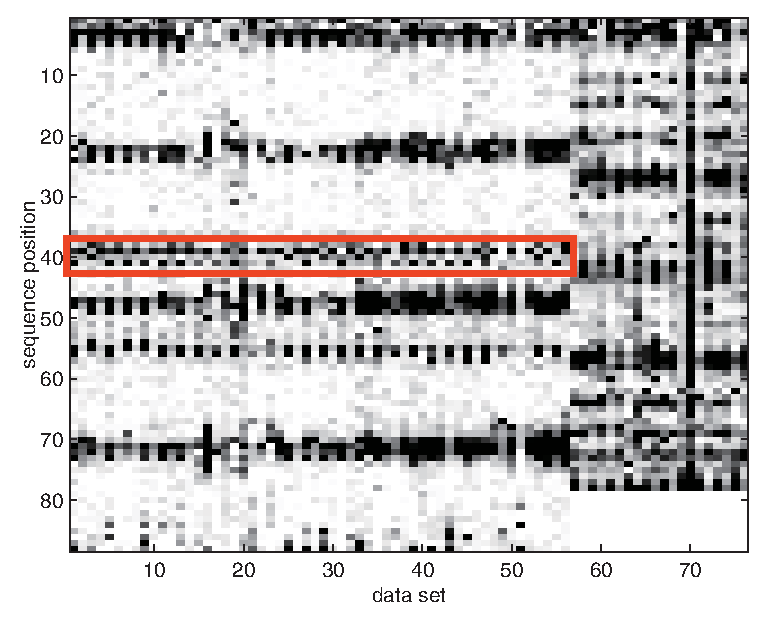
\includegraphics[width=\linewidth]{../figures/eterna_comparison}
\caption{Reactivity results from CE analysis and illumina-based sequencing experiments, over 38 data sets. The heatmap presents results from two methods alternatingly from left to right; CE analysis results are presented on odd numbered x-positions and MySeq results are shown on even numbered x-positions.}
\label{f:eterna_comparison}
\end{figure}
%%%%%%%%%%%%%%%%%%%%%%%%%%%%%%%%%%%%%%%%%%%%%%%%%%%%%%%%%%%%%%%%%%%%%%%%%%%%%%%%

\section{ADDITIONAL DETAILS AND RESULTS}

\subsection{ Rectification step in the preparation of reference band location }
As discussed in Section 3.1, the reference band locations were prepared by manual annotation followed by the rectification step where possible human errors are discovered and corrected through a comparison between two separate experiments. One example of such process is well illustrated by Figure~\ref{f:eterna_comparison}. Visual inspection suggests that in the rectangular region, CE analysis and MySeq consistently show the highest intensity at residue 41 and 39 respectively. This discrepancy gave us an inkling of inaccurate determination of band locations around the corresponding sequence position, leading to rectification of such errors.


\subsection{ Band annotation over all prepared data sets }
The accuracy of band locations determined by the proposed method was discussed and assessed with 95 data sets in Section 3.1 and with additional data sets in Section 3.5. All the results from experiments in Section 3.1 and Section 3.5 are provided respectively in Table~\ref{t:95_data_sets} and in Table~\ref{t:additional_data_sets}.



%%%%%%%%%%%%%%%%%%%%%%%%%%%%%%%%%%%%%%%%%%%%%%%%%%%%%%%%%%%%%%%%%%%%%%%%%%%%%%%%
% OLD VS NEW
%%%%%%%%%%%%%%%%%%%%%%%%%%%%%%%%%%%%%%%%%%%%%%%%%%%%%%%%%%%%%%%%%%%%%%%%%%%%%%%%
\begin{figure}
\centering
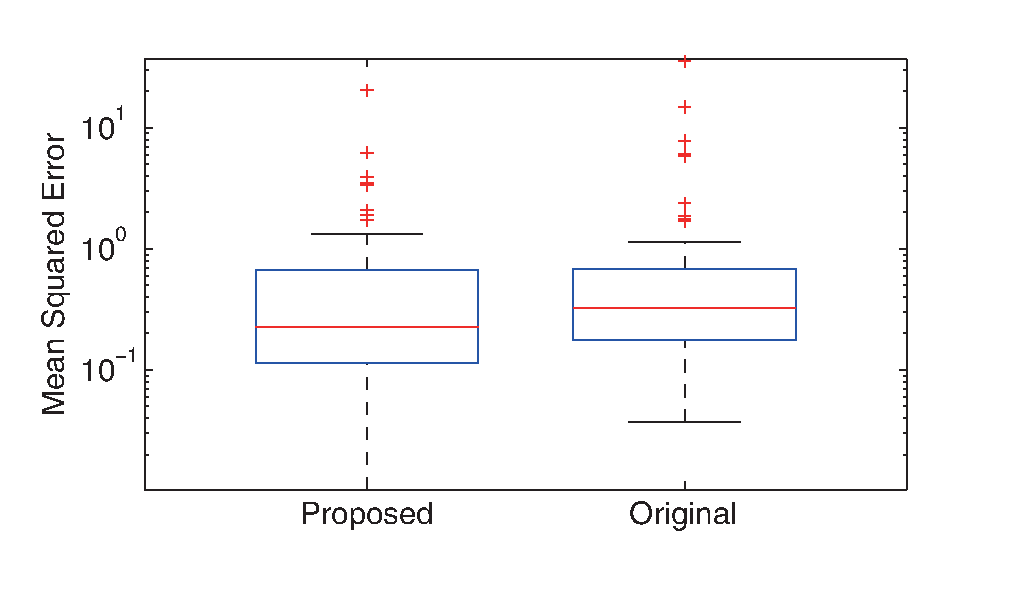
\includegraphics[width=\linewidth]{../figures/supp_old_new_comparison}
\caption{The distribution of MSE for the results from the proposed method and the old method respectively, over the 95 data sets.}
\label{f:old_vs_new}
\end{figure}
%%%%%%%%%%%%%%%%%%%%%%%%%%%%%%%%%%%%%%%%%%%%%%%%%%%%%%%%%%%%%%%%%%%%%%%%%%%%%%%%


\subsection{ Proposed method vs. Earlier HiTrace band annotation method }
With $\escore$-score as a quality indicator for its results, the proposed method becomes more practical compared to the original method provided by HiTrace-Web~\citep{Kim2013}. Furthermore, the accuracy of results improved (about 40\% in terms of median MSE) in the proposed method as shown in Figure~\ref{f:old_vs_new}.


\subsection{ Peak-area quantification experiment results }
The influence of accuracy in band annotation on the results of peak deconvolution was discussed in Section 3.3 and a representative result was presented in Fig.4. All the results are listed in Table~\ref{t:peak_deconvolution}.





\onecolumn

%%%%%%%%%%%%%%%%%%%%%%%%%%%%%%%%%%%%%%%%%%%%%%%%%%%%%%%%%%%%%%%%%%%%%%%%%%%%%%%
% TABLE: 95 DATA SETS RESULT
%%%%%%%%%%%%%%%%%%%%%%%%%%%%%%%%%%%%%%%%%%%%%%%%%%%%%%%%%%%%%%%%%%%%%%%%%%%%%%%

\begin{center}
\begin{longtable}{l ccc}

\caption{Name of data set and corresponding results respectively from the proposed method and QuShape, along with $\escore$-score.} \label{t:95_data_sets} \\
 & & \multicolumn{2}{c}{MSE} \\
Data Set Name & $\escore$-score & \multicolumn{1}{c}{proposed} & QuShape \\\hline
\endfirsthead

%\multicolumn{4}{l}{\textit{Continued from previous page}} \\
 & & \multicolumn{2}{c}{MSE} \\
Data Set Name & $\escore$-score & \multicolumn{1}{c}{proposed} & QuShape \\\hline
\endhead

\\
\multicolumn{4}{r}{\textit{Continued on next page}} \\
\endfoot
\endlastfoot


Fragments of Old Winners		&1.00	&0.82	&2.38 \\
FNM Apatamet 1st try			&1.00 	&0.57 	&0.86 \\
Freywa - Cross FMN - Reshiram	&1.00 	&0.24 	&0.68 \\
wisdave's apatamer \#1			&1.00 	&0.26 	&0.38 \\
Fiskers single aptamer 2		&0.93 	&1.43 	&1.49 \\
Starry's Single III			&1.00 	&0.11 	&1.78 \\
fold vs shapes				&1.00 	&0.18 	&0.15 \\
ViennaRNA design 01			&0.84 	&0.58 	&0.74 \\
ViennaRNA design 03			&0.95 	&0.15 	&1.11 \\
ViennaRNA design 04			&1.00 	&0.09 	&0.33 \\
NUPACK design 02				&0.58 	&4.60 	&66.49 \\
NUPACK design 04				&0.75 	&3.18 	&1.88 \\
Freywa - Cross FMN R2 - Zekrom	&0.96 	&0.98 	&1.10 \\
Tadpole 2.0					&1.00 	&0.10 	&0.46 \\
Kiwi							&1.00 	&0.11 	&0.51 \\
LROppy 93.4\% FMN				&0.97 	&0.09 	&1.26 \\
EteRNA ensemble design 01 (L2)	&0.73 	&4.27 	&4.95 \\
EteRNA ensemble design 02 (L2)	&1.00 	&0.19 	&7.60 \\
EteRNA ensemble design 03 (L2)	&0.94 	&0.22 	&0.74 \\
EteRNA ensemble design 04 (L2)	&0.94 	&0.39 	&0.34 \\
EteRNA ensemble design 05 (sparse 5)		&0.97 	&0.17 	&0.55 \\
EteRNA ensemble design 06 (sparse 5)		&0.91 	&0.58 	&1.70 \\
EteRNA ensemble design 07 (sparse 5)		&0.97 	&0.37 	&6.38 \\
EteRNA ensemble design 08 (sparse 5)		&0.94 	&0.75 	&0.18 \\
EteRNA ensemble design 09 (conventional)		&0.94 	&1.69 	&1.06 \\
EteRNA ensemble design 10 (conventional)		&0.85 	&1.01 	&1.48 \\
EteRNA ensemble design 11 (conventional)		&0.97 	&0.17 	&0.58 \\
EteRNA ensemble design 12 (conventional)		&1.00 	&0.23 	&0.36 \\
Brourd - FMNA 1			&1.00 	&0.09 	&0.40 \\
The Revolution of the Mobile Archer	&1.00 	&0.19 	&0.75 \\
Fragments of old Winners (3)	&0.90 	&0.77 	&5.13 \\
Smart Solution				&1.00 	&0.06 	&0.07 \\
Lump In My Throat				&0.94 	&0.75 	&7.12 \\
JP-14-0-17 (FMN-SBS II)		&0.94 	&0.33 	&0.30 \\
SBSII-2						&0.87 	&0.53 	&6.44 \\
Mod of Quasispecies design Fragments of old winners	&0.87 	&0.47 	&7.35 \\
NUPACK design 01				&0.74 	&21.05 	&62.22 \\
NUPACK design 02				&0.87 	&1.71 	&16.09 \\
NUPACK design 03				&0.90 	&0.84 	&46.15 \\
NUPACK design 04				&0.77 	&1.09 	&5.58 \\
ViennaRNA design 01			&0.81 	&0.28 	&0.51 \\
ViennaRNA design 02			&0.84 	&0.29 	&0.36 \\
ViennaRNA design 03			&0.84 	&0.15 	&0.84 \\
NUPACK design 01				&0.81 	&0.39 	&0.20 \\
NUPACK design 02				&0.87 	&1.30 	&3.30 \\
NUPACK design 03				&0.77 	&1.18 	&0.34 \\
NUPACK design 04				&0.81 	&1.68 	&0.72 \\
ViennaRNA design 01			&0.77 	&3.99 	&0.67 \\
ViennaRNA design 03			&0.81 	&0.06 	&0.25 \\
Fragments of Old Winners (4)	&1.00 	&0.09 	&0.21 \\
GOOD SOLUTION					&1.00 	&0.16 	&0.57 \\
Mod of Quasispecies design Fragments of old winners v2		&0.87 	&0.97 	&10.48 \\
Combo - improved				&1.00 	&0.13 	&0.30 \\
EteRNA ensemble design 0 (sparse 5) 		&1.00 	&0.09 	&0.59 \\
EteRNA ensemble design 1 (sparse 5)		&0.97 	&0.21 	&0.75 \\
EteRNA ensemble design 2 (sparse 5)		&1.00 	&0.17 	&0.75 \\
EteRNA ensemble design 3 (sparse 5)		&0.97 	&0.06 	&0.28 \\
EteRNA ensemble design 4 (L2)		&1.00 	&0.03 	&0.20 \\
EteRNA ensemble design 5 (L2)		&0.94 	&0.33 	&0.78 \\
EteRNA ensemble design 6 (L2)		&0.97 	&0.14 	&0.68 \\
EteRNA ensemble design 7 (L2)		&1.00 	&0.18 	&0.34 \\
EteRNA ensemble design 08 (conventional)		&1.00 	&0.05 	&0.21 \\
EteRNA ensemble design 09 (conventional)		&0.97 	&0.14 	&0.66 \\
EteRNA ensemble design 10 (conventional)		&0.97 	&0.58 	&0.65 \\
EteRNA ensemble design 11 (conventional)		&1.00 	&0.15 	&0.27 \\
Wild Cross - 	2				&0.94 	&0.11 	&0.72 \\
Mod of JerryP70				&1.00 	&0.07 	&0.55 \\
Mod of brourds 1 st round -		&0.84 	&0.13 	&0.88 \\
Unique Stacks					&0.93 	&0.22 	&0.54 \\
G-C pairs in multloops in same direction		&0.95 	&0.02 	&1.38 \\
Fisker's Binding branches		&0.93 	&0.11 	&0.76 \\
NUPACK design 01				&0.95 	&0.27 	&0.93 \\
NUPACK design 02				&0.90 	&0.52 	&0.39 \\
NUPACK design 03				&0.95 	&2.73 	&1.41 \\
NUPACK design 04				&0.98 	&0.38 	&0.39 \\
ViennaRNA design 04			&0.90 	&0.41 	&0.48 \\
EteRNA ensemble design 02 (conventional)		&0.95 	&1.80 	&1.35 \\
EteRNA ensemble design 04 (conventional)		&1.00 	&0.03 	&0.45 \\
EteRNA ensemble design 05 (sparse 5)		&1.00 	&0.06 	&0.05 \\
EteRNA ensemble design 06 (sparse 5)		&1.00 	&0.27 	&0.41 \\
EteRNA ensemble design 07 (sparse 5)		&0.99 	&0.20 	&0.39 \\
EteRNA ensemble design 08 (sparse 5)		&1.00 	&0.12 	&0.10 \\
EteRNA ensemble design 09 (L2)		&0.99 	&0.28 	&13.50 \\
EteRNA ensemble design 11 (L2)		&0.98 	&0.21 	&0.18 \\
EteRNA ensemble design 12 (L2)		&0.99 	&0.08 	&0.23 \\
UUU / GCA Triloops (Round 2)	&0.85 	&0.51 	&3.00 \\
Uracil in 1-2 x2				&0.85 	&0.12 	&0.79 \\
1 U-leg, 1 A-leg				&0.94 	&1.19 	&3.98 \\
Bonus Army					&0.85 	&0.39 	&0.86 \\
wisdave's 2nd round			&0.82 	&0.74 	&1.02 \\
C - BACK						&0.85 	&1.19 	&0.24 \\
Beauty in Balance				&0.89 	&1.36 	&1.33 \\
Very Low Entropy <0.6 T-B-C \#5	&0.88 	&0.14 	&0.16 \\
Improves on Quasispecies UUU/GCA Triloop	&0.91 	&0.08 	&0.06 \\
sta1							&0.79 	&0.23 	&1.86 \\

\end{longtable}
\end{center}



\newpage



%%%%%%%%%%%%%%%%%%%%%%%%%%%%%%%%%%%%%%%%%%%%%%%%%%%%%%%%%%%%%%%%%%%%%%%%%%%%%%%
% TABLE: ADDITIONAL, LONGER DATA RESULT
%%%%%%%%%%%%%%%%%%%%%%%%%%%%%%%%%%%%%%%%%%%%%%%%%%%%%%%%%%%%%%%%%%%%%%%%%%%%%%%

\begin{center}
\begin{longtable}{l cccc}

\caption{Description of longer data sets and results from the tests with these data sets. $^a$An extraordinary result mainly caused by a misalignment between profiles.} \label{t:additional_data_sets} \\

Name & \# profiles & \# bands per profile & MSE & $\escore$-score \\
\hline
\endfirsthead
Name & \# profiles & \# bands per profile & MSE & $\escore$-score \\
\endhead
\endfoot
%{$^a$An extraordinary result mainly caused by a misalignment between profiles (to be discussed in the discussion section) }
\endlastfoot

GIR1 noref 	& 21 & 199 & 0.09 & 0.99 \\
GIR1 ref 		& 21 & 225 & 0.12 & 0.98 \\
AdoCbl noref 	& 16 & 179 & 0.61 & 0.97 \\
AdoCbl ref 	& 16 & 205 & 0.68 & 0.90 \\
VS noref 		& 48 & 195 & 0.16 & 0.96 \\
VS ref 		& 48 & 233 & 0.12 & 0.96 \\
SAM noref 	& 32 & 103 & 0.09 & 0.96 \\
SAM ref 		& 32 & 143 & 0.09 & 0.96 \\
HTP noref 	& 32 & 79  & 0.05 & 1.00 \\
HTP ref 		& 32 & 116 & 0.05 & 1.00 \\
Tbox 		& 20 & 141 & 0.34 & 0.98 \\
tRNA 		& 20 & 119 & 0.63 & 0.83 \\
cdiAMP 		& 36 & 171 & 0.16 & 0.99 \\
16S 			& 8  & 125 & 0.21 & 0.98 \\
C19 			& 16 & 319 & 0.18 & 0.99 \\
tC19 		& 16 & 248 & 0.01 & 1.00 \\
tC19Z 		& 16 & 248 & 0.01 & 0.99 \\
C1Lig 		& 7  & 167 & 0.04 & 1.00 \\
Hox5 		& 9  & 261 & 0.11 & 0.99 \\
Hox9D 		& 16 & 296 & 0.44 & 0.99 \\
L-21			& 20 & 413 & 2.00$^a$ & 0.98 \\
\end{longtable}
\end{center}



\newpage


%%%%%%%%%%%%%%%%%%%%%%%%%%%%%%%%%%%%%%%%%%%%%%%%%%%%%%%%%%%%%%%%%%%%%%%%%%%%%%%
% TABLE: PEAK DECONVOLUTION
%%%%%%%%%%%%%%%%%%%%%%%%%%%%%%%%%%%%%%%%%%%%%%%%%%%%%%%%%%%%%%%%%%%%%%%%%%%%%%%

\begin{center}
\begin{longtable}{l ccc}

\caption{Name of data set and corresponding results respectively from the proposed method and manual annotation, along with the ratio between two MSE values (proposed / manual)} \label{t:peak_deconvolution} \\
 & & \multicolumn{2}{c}{MSE} \\
Data Set Name & ratio & \multicolumn{1}{c}{proposed} & manual \\\hline
\endfirsthead

%\multicolumn{4}{l}{\textit{Continued from previous page}} \\
 & & \multicolumn{2}{c}{MSE} \\
Data Set Name & ratio & \multicolumn{1}{c}{proposed} & manual \\\hline
\endhead

\\
\multicolumn{4}{r}{\textit{Continued on next page}} \\
\endfoot
\endlastfoot


Fragments of Old Winners		&1.15	&0.82	&0.71 \\
FNM Apatamet 1st try			&0.94 	&0.57 	&0.61 \\
Freywa - Cross FMN - Reshiram	&2.60 	&0.24 	&0.09 \\
wisdave's apatamer \#1			&1.32 	&0.26 	&0.20 \\
Fiskers single aptamer 2		&9.31 	&1.43 	&0.15 \\
Starry's Single III			&0.73 	&0.11 	&0.15 \\
fold vs shapes				&1.22 	&0.18 	&0.15 \\
ViennaRNA design 01			&0.97 	&0.58 	&0.60 \\
ViennaRNA design 03			&0.67 	&0.15 	&0.22 \\
ViennaRNA design 04			&1.04 	&0.09 	&0.09 \\
NUPACK design 02				&3.80 	&4.60 	&1.21 \\
NUPACK design 04				&10.10 	&3.18 	&0.32 \\
Freywa - Cross FMN R2 - Zekrom	&3.31	&0.98 	&0.30 \\
Tadpole 2.0					&1.77 	&0.10 	&0.06 \\
Kiwi							&4.07 	&0.11 	&0.03 \\
LROppy 93.4\% FMN				&2.07 	&0.09 	&0.04 \\
EteRNA ensemble design 01 (L2)	&5.33 	&4.27 	&0.80 \\
EteRNA ensemble design 02 (L2)	&3.03 	&0.19 	&0.06 \\
EteRNA ensemble design 03 (L2)	&1.12 	&0.22 	&0.19 \\
EteRNA ensemble design 04 (L2)	&1.47 	&0.39 	&0.26 \\
EteRNA ensemble design 05 (sparse 5)		&2.51 	&0.17 	&0.07 \\
EteRNA ensemble design 06 (sparse 5)		&1.91 	&0.58 	&0.31 \\
EteRNA ensemble design 07 (sparse 5)		&0.83 	&0.37 	&0.44 \\
EteRNA ensemble design 08 (sparse 5)		&5.90 	&0.75 	&0.13 \\
EteRNA ensemble design 09 (conventional)		&13.01 	&1.69 	&0.13 \\
EteRNA ensemble design 10 (conventional)		&1.16 	&1.01 	&0.87 \\
EteRNA ensemble design 11 (conventional)		&1.86 	&0.17 	&0.09 \\
EteRNA ensemble design 12 (conventional)		&2.51 	&0.23 	&0.09 \\
UUU / GCA Triloops (Round 2)	&40.59 	&0.51 	&0.01 \\
Uracil in 1-2 x2				&1.20 	&0.12 	&0.10 \\
1 U-leg, 1 A-leg				&3.62 	&1.19 	&0.33 \\
Bonus Army					&1.61 	&0.39 	&0.21 \\
wisdave's 2nd round			&12.73 	&0.74 	&0.06 \\
C - BACK						&2.75	&1.19 	&0.43 \\
Beauty in Balance				&9.22 	&1.36 	&0.15 \\
Very Low Entropy <0.6 T-B-C \#5	&1.36 	&0.14 	&0.11 \\
Improves on Quasispecies UUU/GCA Triloop	&11.22 	&0.08 	&0.01 \\
sta1							&1.09 	&0.23 	&0.21 \\

\end{longtable}
\end{center}





\newpage


%%%%%%%%%%%%%%%%%%%%%%%%%%%%%%%%%%%%%%%%%%%%%%%%%%%%%%%%%%%%%%%%%%%%%%%%%%%%%%%
% TABLE 3
%%%%%%%%%%%%%%%%%%%%%%%%%%%%%%%%%%%%%%%%%%%%%%%%%%%%%%%%%%%%%%%%%%%%%%%%%%%%%%%

\begin{center}
\begin{longtable}{lccc}

\caption{Name and type of data profile, and the Pearson's correlation coefficients between manually quantified areas, and those quantified by the proposed method and by QuShape respectively. Average values are posted for the multiple results from repetitive experiments with same data.} \\
 & & \multicolumn{2}{c}{correlation (averaged)} \\
Data Set Name & Data Type & proposed & QuShape \\\hline
\endfirsthead

%\multicolumn{4}{l}{\textit{Continued from previous page}} \\
 & & \multicolumn{2}{c}{correlation (averaged)} \\
Data Set Name & Data Type & proposed & QuShape \\\hline
\endhead

\\
\multicolumn{4}{r}{\textit{Continued on next page}} \\
\endfoot
\endlastfoot

Fragments of Old Winners	&	DMS	&	0.9389 	&	0.9654 	\\
FNM Apatamet 1st try	&	DMS	&	0.6913 	&	0.9468 	\\
Freywa - Cross FMN - Reshiram	&	DMS	&	0.9734 	&	0.9433 	\\
wisdave's apatamer \#1	&	DMS	&	0.9796 	&	0.9546 	\\
Fiskers single aptamer 2	&	DMS	&	0.9710 	&	0.9588 	\\
Starry's Single III	&	DMS	&	0.9788 	&	0.7297 	\\
fold vs shapes	&	DMS	&	0.9898 	&	0.9880 	\\
ViennaRNA design 01	&	DMS	&	0.9932 	&	0.9745 	\\
ViennaRNA design 03	&	DMS	&	0.9965 	&	0.9929 	\\
ViennaRNA design 04	&	DMS	&	0.9697 	&	0.9232 	\\
NUPACK design 02	&	DMS	&	0.9180 	&	0.8848 	\\
NUPACK design 04	&	DMS	&	0.9539 	&	0.7359 	\\
Freywa - Cross FMN R2 - Zekrom	&	DMS	&	0.9816 	&	0.7436 	\\
Tadpole 2.0	&	DMS	&	0.9764 	&	0.9444 	\\
Kiwi	&	DMS	&	0.9964 	&	0.8889 	\\
LROppy 93.4\% FMN	&	DMS	&	0.9901 	&	0.9422 	\\
EteRNA ensemble design 01 (L2)	&	DMS	&	0.9863 	&	0.9917 	\\
EteRNA ensemble design 02 (L2)	&	DMS	&	0.9643 	&	0.8977 	\\
EteRNA ensemble design 03 (L2)	&	DMS	&	0.9198 	&	0.9130 	\\
EteRNA ensemble design 04 (L2)	&	DMS	&	0.9175 	&	0.9482 	\\
EteRNA ensemble design 05 (sparse 5)	&	DMS	&	0.9676 	&	0.9616 	\\
EteRNA ensemble design 06 (sparse 5)	&	DMS	&	0.9894 	&	0.9822 	\\
EteRNA ensemble design 07 (sparse 5)	&	DMS	&	0.9499 	&	0.8044 	\\
EteRNA ensemble design 08 (sparse 5)	&	DMS	&	0.9508 	&	0.9748 	\\
EteRNA ensemble design 09 (conventional)	&	DMS	&	0.5388 	&	0.6876 	\\
EteRNA ensemble design 10 (conventional)	&	DMS	&	0.9898 	&	0.9867 	\\
EteRNA ensemble design 11 (conventional)	&	DMS	&	0.9918 	&	0.9480 	\\
EteRNA ensemble design 12 (conventional)	&	DMS	&	0.9763 	&	0.9109 	\\
Brourd - FMNA 1	&	SHAPE	&	0.9733 	&	0.9480 	\\
Brourd - FMNA 1	&	DMS	&	0.9907 	&	0.7227 	\\
The Revolution of the Mobile Archer	&	SHAPE	&	0.9891 	&	0.9360 	\\
The Revolution of the Mobile Archer	&	DMS	&	0.9814 	&	0.9785 	\\
Fragments of old Winners (3)	&	SHAPE	&	0.9943 	&	0.9756 	\\
Fragments of old Winners (3)	&	DMS	&	0.9980 	&	0.9868 	\\
Smart Solution	&	SHAPE	&	0.9898 	&	0.9883 	\\
Smart Solution	&	DMS	&	0.9941 	&	0.8834 	\\
Lump In My Throat	&	SHAPE	&	0.9530 	&	0.9545 	\\
Lump In My Throat	&	DMS	&	0.9887 	&	0.7225 	\\
JP-14-0-17 (FMN-SBS II)	&	SHAPE	&	0.9436 	&	0.9762 	\\
JP-14-0-17 (FMN-SBS II)	&	DMS	&	0.9803 	&	0.9684 	\\
SBSII-2	&	SHAPE	&	0.9192 	&	0.9057 	\\
SBSII-2	&	DMS	&	0.9571 	&	0.9093 	\\
Mod of Quasispecies design Fragments of old winners	&	SHAPE	&	0.9417 	&	0.9724 	\\
Mod of Quasispecies design Fragments of old winners	&	DMS	&	0.9631 	&	0.4340 	\\
NUPACK design 01	&	SHAPE	&	0.9683 	&	0.9706 	\\
NUPACK design 01	&	DMS	&	0.9860 	&	0.9842 	\\
NUPACK design 02	&	SHAPE	&	0.8134 	&	0.5124 	\\
NUPACK design 02	&	DMS	&	0.9185 	&	0.4406 	\\
NUPACK design 03	&	SHAPE	&	0.9476 	&	0.9102 	\\
NUPACK design 03	&	DMS	&	0.9987 	&	0.9978 	\\
NUPACK design 04	&	SHAPE	&	0.9994 	&	0.9898 	\\
NUPACK design 04	&	DMS	&	0.9994 	&	0.9657 	\\
ViennaRNA design 01	&	SHAPE	&	0.9206 	&	0.7119 	\\
ViennaRNA design 01	&	DMS	&	0.9831 	&	0.5016 	\\
ViennaRNA design 02	&	SHAPE	&	0.8999 	&	0.7067 	\\
ViennaRNA design 02	&	DMS	&	0.9789 	&	0.6991 	\\
ViennaRNA design 03	&	SHAPE	&	0.8780 	&	0.7357 	\\
ViennaRNA design 03	&	DMS	&	0.9726 	&	0.7832 	\\
NUPACK design 01	&	SHAPE	&	0.8582 	&	0.8934 	\\
NUPACK design 01	&	DMS	&	0.9913 	&	0.9948 	\\
NUPACK design 02	&	SHAPE	&	0.8971 	&	0.7229 	\\
NUPACK design 02	&	DMS	&	0.9497 	&	0.9425 	\\
NUPACK design 03	&	SHAPE	&	0.6857 	&	0.8557 	\\
NUPACK design 03	&	DMS	&	0.9487 	&	0.9545 	\\
NUPACK design 04	&	SHAPE	&	0.9626 	&	0.7790 	\\
NUPACK design 04	&	DMS	&	0.9923 	&	0.8958 	\\
ViennaRNA design 01	&	SHAPE	&	0.9422 	&	0.7428 	\\
ViennaRNA design 01	&	DMS	&	0.9714 	&	0.9098 	\\
ViennaRNA design 03	&	SHAPE	&	0.9907 	&	0.9231 	\\
ViennaRNA design 03	&	DMS	&	0.9954 	&	0.9144 	\\
Fragments of Old Winners (4)	&	SHAPE	&	0.9742 	&	0.9742 	\\
Fragments of Old Winners (4)	&	DMS	&	0.9932 	&	0.9890 	\\
GOOD SOLUTION	&	SHAPE	&	0.9514 	&	0.9355 	\\
GOOD SOLUTION	&	DMS	&	0.9840 	&	0.9714 	\\
Mod of Quasispecies design Fragments of old winners v2	&	SHAPE	&	0.5959 	&	0.6670 	\\
Mod of Quasispecies design Fragments of old winners v2	&	DMS	&	0.5214 	&	0.9051 	\\
Combo - improved	&	SHAPE	&	0.9482 	&	0.9111 	\\
Combo - improved	&	DMS	&	0.9962 	&	0.9854 	\\
EteRNA ensemble design 0 (sparse 5)	&	SHAPE	&	0.9483 	&	0.9265 	\\
EteRNA ensemble design 0 (sparse 5)	&	DMS	&	0.9800 	&	0.8917 	\\
EteRNA ensemble design 1 (sparse 5)	&	SHAPE	&	0.9159 	&	0.9152 	\\
EteRNA ensemble design 1 (sparse 5)	&	DMS	&	0.9540 	&	0.9228 	\\
EteRNA ensemble design 2 (sparse 5)	&	SHAPE	&	0.9390 	&	0.9145 	\\
EteRNA ensemble design 2 (sparse 5)	&	DMS	&	0.9597 	&	0.9029 	\\
EteRNA ensemble design 3 (sparse 5)	&	SHAPE	&	0.9960 	&	0.9217 	\\
EteRNA ensemble design 3 (sparse 5)	&	DMS	&	0.9967 	&	0.9216 	\\
EteRNA ensemble design 4 (L2)	&	SHAPE	&	0.9947 	&	0.9172 	\\
EteRNA ensemble design 4 (L2)	&	DMS	&	0.9878 	&	0.9782 	\\
EteRNA ensemble design 5 (L2)	&	SHAPE	&	0.5964 	&	0.4973 	\\
EteRNA ensemble design 5 (L2)	&	DMS	&	0.8830 	&	0.8574 	\\
EteRNA ensemble design 6 (L2)	&	SHAPE	&	0.9790 	&	0.9049 	\\
EteRNA ensemble design 6 (L2)	&	DMS	&	0.9884 	&	0.8338 	\\
EteRNA ensemble design 7 (L2)	&	SHAPE	&	0.9613 	&	0.9730 	\\
EteRNA ensemble design 7 (L2)	&	DMS	&	0.9503 	&	0.9526 	\\
EteRNA ensemble design 08 (conventional)	&	SHAPE	&	0.9904 	&	0.9249 	\\
EteRNA ensemble design 08 (conventional)	&	DMS	&	0.9948 	&	0.9326 	\\
EteRNA ensemble design 09 (conventional)	&	SHAPE	&	0.9413 	&	0.9193 	\\
EteRNA ensemble design 09 (conventional)	&	DMS	&	0.9936 	&	0.9218 	\\
EteRNA ensemble design 10 (conventional)	&	SHAPE	&	0.6216 	&	0.8549 	\\
EteRNA ensemble design 10 (conventional)	&	DMS	&	0.9644 	&	0.9046 	\\
EteRNA ensemble design 11 (conventional)	&	SHAPE	&	0.9857 	&	0.9857 	\\
EteRNA ensemble design 11 (conventional)	&	DMS	&	0.9887 	&	0.9845 	\\
Wild Cross - 2	&	SHAPE	&	0.9767 	&	0.7966 	\\
Wild Cross - 2	&	DMS	&	0.9860 	&	0.9414 	\\
Mod of JerryP70	&	SHAPE	&	0.9576 	&	0.9068 	\\
Mod of JerryP70	&	DMS	&	0.9957 	&	0.7095 	\\
Mod of brourds 1 st round -	&	SHAPE	&	0.9992 	&	0.8678 	\\
Mod of brourds 1 st round -	&	DMS	&	0.9998 	&	0.9901 	\\
Unique Stacks	&	SHAPE	&	0.9680 	&	0.8632 	\\
Unique Stacks	&	DMS	&	0.9862 	&	0.8142 	\\
G-C pairs in multloops in same direction	&	SHAPE	&	0.9948 	&	0.9698 	\\
G-C pairs in multloops in same direction	&	DMS	&	0.9991 	&	0.9866 	\\
Fisker's Binding branches	&	SHAPE	&	0.3851 	&	0.9764 	\\
Fisker's Binding branches	&	DMS	&	0.2767 	&	0.9424 	\\
NUPACK design 01	&	SHAPE	&	0.9885 	&	0.9591 	\\
NUPACK design 01	&	DMS	&	0.9920 	&	0.9836 	\\
NUPACK design 02	&	SHAPE	&	0.8843 	&	0.8366 	\\
NUPACK design 02	&	DMS	&	0.9646 	&	0.8545 	\\
NUPACK design 03	&	SHAPE	&	0.8027 	&	0.7560 	\\
NUPACK design 03	&	DMS	&	0.9574 	&	0.7813 	\\
NUPACK design 04	&	SHAPE	&	0.7613 	&	0.9667 	\\
NUPACK design 04	&	DMS	&	0.9245 	&	0.9888 	\\
ViennaRNA design 04	&	SHAPE	&	0.8822 	&	0.8842 	\\
ViennaRNA design 04	&	DMS	&	0.9935 	&	0.9872 	\\
EteRNA ensemble design 02 (conventional)	&	SHAPE	&	0.9468 	&	0.9561 	\\
EteRNA ensemble design 02 (conventional)	&	DMS	&	0.8877 	&	0.8607 	\\
EteRNA ensemble design 04 (conventional)	&	SHAPE	&	0.9814 	&	0.9433 	\\
EteRNA ensemble design 04 (conventional)	&	DMS	&	0.9903 	&	0.7494 	\\
EteRNA ensemble design 05 (sparse 5)	&	SHAPE	&	0.8983 	&	0.9915 	\\
EteRNA ensemble design 05 (sparse 5)	&	DMS	&	0.9931 	&	0.9961 	\\
EteRNA ensemble design 06 (sparse 5)	&	SHAPE	&	0.9553 	&	0.5474 	\\
EteRNA ensemble design 06 (sparse 5)	&	DMS	&	0.9615 	&	0.9208 	\\
EteRNA ensemble design 07 (sparse 5)	&	SHAPE	&	0.9886 	&	0.9736 	\\
EteRNA ensemble design 07 (sparse 5)	&	DMS	&	0.9343 	&	0.9637 	\\
EteRNA ensemble design 08 (sparse 5)	&	SHAPE	&	0.9814 	&	0.9753 	\\
EteRNA ensemble design 08 (sparse 5)	&	DMS	&	0.9775 	&	0.9060 	\\
EteRNA ensemble design 09 (L2)	&	SHAPE	&	0.9468 	&	0.9359 	\\
EteRNA ensemble design 09 (L2)	&	DMS	&	0.8991 	&	0.5745 	\\
EteRNA ensemble design 11 (L2)	&	SHAPE	&	0.8985 	&	0.9365 	\\
EteRNA ensemble design 11 (L2)	&	DMS	&	0.9389 	&	0.8063 	\\
EteRNA ensemble design 12 (L2)	&	SHAPE	&	0.9781 	&	0.9616 	\\
EteRNA ensemble design 12 (L2)	&	DMS	&	0.9633 	&	0.9511 	\\
UUU / GCA Triloops (Round 2)	&	SHAPE	&	0.9896 	&	0.8104 	\\
Uracil in 1-2 x2	&	SHAPE	&	0.9808 	&	0.9665 	\\
1 U-leg, 1 A-leg	&	SHAPE	&	0.8221 	&	0.6919 	\\
Bonus Army	&	SHAPE	&	0.9763 	&	0.7612 	\\
wisdave's 2nd round	&	SHAPE	&	0.9739 	&	0.8770 	\\
C - BACK	&	SHAPE	&	0.9419 	&	0.9441 	\\
Beauty in Balance	&	SHAPE	&	0.9391 	&	0.7477 	\\
Very Low Entropy <0.6 T-B-C \#5	&	SHAPE	&	0.9615 	&	0.8384 	\\
Improves on Quasispecies UUU/GCA Triloop	&	SHAPE	&	0.9885 	&	0.9971 	\\
sta1	&	SHAPE	&	0.9956 	&	0.9117 	\\




\end{longtable}
\end{center}







\twocolumn









\bibliographystyle{natbib}
%\bibliographystyle{reference}
%\bibliographystyle{unsrt}
\bibliography{reference}


\end{document}


